
\documentclass[12pt]{report}
\usepackage{textcomp}

\addtolength{\hoffset}{-2.25cm}
\addtolength{\textwidth}{4.5cm}
\addtolength{\voffset}{-2.5cm}
\addtolength{\textheight}{5cm}
\setlength{\parskip}{0pt}
\setlength{\parindent}{15pt}

\usepackage{graphicx}
\graphicspath{ {./images/} }

\usepackage{amsthm}
\usepackage{amsmath}
\usepackage{amssymb}

\usepackage[colorlinks = true, linkcolor = black, citecolor = black, final]{hyperref}

\usepackage{graphicx}
\usepackage{multicol}
\usepackage{marvosym}
\usepackage{wasysym}

\usepackage{outlines}
\usepackage[utf8]{inputenc}
\usepackage[english]{babel}

\usepackage{enumitem,amssymb}

\newcommand{\pr}[1]{\left(#1\right)}

\usepackage{pgfplots}
\pgfplotsset{compat=1.16}
\usepackage{circuitikz}
\usepackage{tikz}
\usetikzlibrary{patterns}
\usetikzlibrary{arrows.meta}

\setlength{\parindent}{0in}

\pagestyle{plain}

\usepackage{listings}

\definecolor{codegreen}{rgb}{0,0.6,0}
\definecolor{codegray}{rgb}{0.5,0.5,0.5}
\definecolor{codepurple}{rgb}{0.58,0,0.82}
\definecolor{backcolour}{rgb}{0.95,0.95,0.92}
\definecolor{backcolour2}{rgb}{0.44,0.63,0.99}

\definecolor{dkgreen}{rgb}{0,0.6,0}
\definecolor{gray}{rgb}{0.5,0.5,0.5}
\definecolor{mauve}{rgb}{0.58,0,0.82}

\lstset{
    language=Verilog,
    breakatwhitespace=false,         
    breaklines=true,                 
    captionpos=b,                    
    keepspaces=true,                 
    numbers=left,                    
    numbersep=5pt,                  
    showspaces=false,                
    showstringspaces=false,
    showtabs=false       
    columns=flexible,
    basicstyle={\small\ttfamily},
    numberstyle=\tiny\color{gray},
    keywordstyle=\color{blue},
    commentstyle=\color{dkgreen},
     % stringstyle=\color{mauve},
    stringstyle=\color{orange},
    backgroundcolor=\color{backcolour},
    tabsize=4  
}

%%%%%%%%%%%%%%%% These commands are taken from Professor Ashmanskas!
\newcommand{\ohm}{\Omega}
\newcommand{\kohm}{{\rm k}\Omega}
\newcommand{\Mohm}{{\rm M}\Omega}
\newcommand{\dif}{{\rm d}}
\newcommand{\kgmps}{{\rm kg\cdot m/s}}
\newcommand{\degC}{{}^\circ{\rm C}}
\newcommand{\degF}{{}^\circ{\rm F}}
\newcommand{\K}{{\rm K}}
\newcommand{\liter}{{\rm L}}
\newcommand{\mL}{{\rm mL}}
\newcommand{\atm}{{\rm atm}}
\newcommand{\mol}{{\rm mol}}
\newcommand{\Cal}{{\rm Cal}}
\newcommand{\W}{{\rm W}}
\newcommand{\kW}{{\rm kW}}
\newcommand{\dB}{{\rm dB}}
\newcommand{\amu}{{\rm u}}
\newcommand{\Pa}{{\rm Pa}}
\newcommand{\J}{{\rm J}}
\newcommand{\N}{{\rm N}}
\newcommand{\pC}{{\rm pC}}
\newcommand{\C}{{\rm C}}
\newcommand{\T}{{\rm T}}
\newcommand{\eV}{{\rm eV}}
\newcommand{\V}{{\rm V}}
\newcommand{\mV}{{\rm mV}}
\newcommand{\Vpp}{{ V}_{ pp}}
\newcommand{\mVpp}{{\rm mV}_{\rm pp}}
\newcommand{\Vac}{{\rm V}_{\rm AC}}
\newcommand{\Vdc}{{\rm V}_{\rm DC}}
\newcommand{\Vbold}{{\bf V}}
\newcommand{\Ibold}{{\bf I}}
\newcommand{\Zbold}{{\bf Z}}
\newcommand{\kV}{{\rm kV}}
\newcommand{\emf}{{\cal E}}
\newcommand{\A}{{\rm A}}
\newcommand{\mA}{{\rm mA}}
\newcommand{\uA}{{\rm \mu A}}
\newcommand{\nA}{{\rm nA}}
\newcommand{\F}{{\rm F}}
\newcommand{\uF}{\mu{\rm F}}
\newcommand{\nF}{{\rm nF}}
\newcommand{\pF}{{\rm pF}}
\newcommand{\mH}{{\rm mH}}
\newcommand{\muH}{{\rm \mu H}}
\newcommand{\uC}{\mu{\rm C}}
\newcommand{\nC}{{\rm nC}}
\newcommand{\MJ}{{\rm MJ}}
\newcommand{\kJ}{{\rm kJ}}
\newcommand{\kg}{{\rm kg}}
\newcommand{\g}{{\rm g}}
\newcommand{\m}{{\rm m}}
\newcommand{\s}{{\rm s}}
\newcommand{\ms}{\rm ms}
\newcommand{\us}{\mu{\rm s}}
\newcommand{\ns}{{\rm ns}}
\newcommand{\cm}{{\rm cm}}
\newcommand{\um}{\mu{\rm m}}
\newcommand{\mm}{{\rm mm}}
\newcommand{\nm}{{\rm nm}}
\newcommand{\km}{{\rm km}}
\newcommand{\G}{{6.67\times10^{-11}~\frac{\N~\m^2}{\kg^2}}}
\newcommand{\mpsps}{\frac{\m}{\s^2}}
\newcommand{\kgmsq}{\kg\cdot\m^2}
\newcommand{\Nm}{\N~\m}      % {\N\cdot\m}
\newcommand{\ihat}{{\hat{i}}}
\newcommand{\jhat}{{\hat{j}}}
\newcommand{\khat}{{\hat{k}}}
\newcommand{\Hz}{{\rm Hz}}
\newcommand{\kHz}{{\rm kHz}}
\newcommand{\MHz}{{\rm MHz}}
\newcommand{\kN}{{\rm kN}}
\newcommand{\red}{\color{red}}
%%%%%%%%%%%%%%%%%%%%%%%%%%

\newcommand{\lst}{\lstinline}
\newcommand{\bs}{\bigskip}
\newcommand{\Vo}{{V}_{out}}
\newcommand{\Vi}{{V}_{in}}

\begin{document}

\bigskip
\bigskip
\bigskip
\bigskip
\begin{titlepage}

   \begin{center}
       \vspace*{2in}

       \textbf{\Huge Forcing a meaninful future: \\ Brain-spine-muscle interfaces\\
       \smallskip }

       \vspace{0.5in}

       {\large By Jackson Powell \\ \small For future Jackson}

    \vspace{1cm}

    \begin{center}
        \textbf{Once you know the way broadly, you can see it in all things.\\
        -- The Book of Five Rings by Miyamoto Musashi}
    
    \end{center}


\vspace{0.5cm}
        
\centerline{\rule{13cm}{0.4pt}}
\tableofcontents
\centerline{\rule{13cm}{0.4pt}}
            
       \vspace{0.8cm}
     
       \end{center}


\end{titlepage}

\pagebreak




{\scshape J. Powell} \hfill {\scshape \large Brain-Spine-Muscle Interfaces} \hfill {\scshape 2023}
 
\smallskip

\hrule
\bigskip
\normalsize 



\section{Overview}

\subsection{Purpose}
The purpose of this book is to aggregate all of the content and tools I will need in forging the future I desire: building better brain-spine-muscle interfaces. 

\subsection{Content}
It is true that total recovery from spinal cord injury, in sever cases, will require both therapeutic and electronic intervention. One must therefore learn of physiology and electronics to be able to solve these problems. I will cover, in some depth, both the electronics, math, and physiology I think I'll need. While programming will likely be an essential tool in this endeavor, I will not discuss programming beyond Verilog (which is an aspect of electronics). This is because programming is something you learn by doing, and writing out C++ algorithms in a PDF would be a waste of time!

\vfill\pagebreak

\part[Electronics]{Electronics
            \vspace{0.2in}
            \begin{center}
            \begin{minipage}[l]{10cm}\small
                Like many of the vagabonds who live in the fields, stray horses seemed to him to be good-natured things. When you're through with them, they ask for nothing; they just go off quietly somewhere by themselves. \newline
                -- Musashi by Eiji Yoshikawa
            \end{minipage}
            \end{center}}

\chapter{Background Information} 

\subsection{Overview} 
The bulk of this information comes from the Lab Electronics course at the University of Pennsylvania, taught to me by Professor Ashmanskas\footnote{\url{https://www.hep.upenn.edu/Classes/Phys364_spring23/}}$^,$\footnote{\url{http://www.hep.upenn.edu/~ashmansk/}}. As a comment on notation: $V$ represents a variable value, while V represents a unit (or at least, that's what it should be; sometimes I forget proper notation). Graphics like this were made using CircuitTikz, whose manual can be found \href{https://texdoc.org/serve/circuitikz/0}{here}.\newline

\section{How Electricity Works} 
\subsection{The misconception} One often represents electricity with the canonical metaphor of water flowing in a tube, equating the flow of water, which powers a wheel of some sort, as being the equivalent of electrons pushing through a wire. Incidentally, this simplifying schema illustrates a key misconception in the nature of electricity. This is easiest exemplified in the mode with which electricity reaches one's house from a power-plant, which before arriving will be subject to breaks in the circuit (transformers). In the traditional viewing of electricity, that which one is taught in early education, this is disconcerting as one would think that if electrons can not physically go from battery to bulb, then how can their kinetic energy be transferred and light it?\newline

When a battery sits without wires attached, around it is an electric field. This field does not dissipate because no electrons flow from it. When wires are attached, charge accumulates on the surface of the wires. This causes a small electric field within the wires, but the drift velocity of electrons within the wire is quite slow---nowhere near the speed of light. However, the flow of electrons within the wire is sufficient to drive an electric field which exists around the wires. From this, we can determine the direction that energy will flow by taking the cross product of the electric and magnetic fields. In fact, if an lightbulb is attached, this means that energy flows from the battery to the bulb in all directions, not through the wires itself.\newline 

Let us consider now what will happen with an AC circuit, where the electromotive force flips with each cycle. In this case, both the electric and magnetic fields switch directions, meaning that their cross product will remain the same and power the lightbulb. Notably, the electrons do not move much (if at all) in this setup---but this is not a surprise, as it is not the electrons that carry the energy anyway. Now, it is still essential to recognize that it is the movement of electrons within the filament of a lightbulb that creates light. This is, indeed, from kinetic energy transferred from electrons bouncing against the metals lattice, dissipating energy in the form of light. The necessary distinction is that it is not electrons that flow all the way from the battery, but rather it is vibrations of those that were, and always will be, within the bulb itself. When you consider it like this, it is straightforward---as the electric field derived from the battery is what provides the electrons with enough kinetic energy to power the bulb.\newline

Interestingly, comparisons to the ``water flow" model fail dramatically in the traditional sense, but the Venturi Effect used to describe fluid flow actually succeeds. In adding a bulb you add a resistor, which is comparable to adding a part of a pipe with a smaller diameter. As water will flow faster in this section of the tube, so too will electrons. In order to maintain the same current as is through the rest of the tube, the drift velocity, $\mathrm{V_d}$, must be higher. $\mathrm{V_d}$ is proportional to the electromotive force, E, meaning the force is highest within the bulb.\newline 

Of course you may say: ``well then why do we use wires at all?" The answer is that wires are helpful in channeling the fields, thereby making them more efficient. Knowing all of this, in this work I will almost invariable describe the flow of current as electrons moving through a wire. This is because it is much easier to think of electricity in this way, hence the ubiquitous misconception. 

\subsection{Nuances in the fields} It is worth explicitly highlighting that the electric field that causes the actual flow is from charges along the wires, rather than the battery. This is notable because if this were not the case, the proximity of the bulb to the battery would dictate its brightness. One may wonder how this type of charge distribution can be established so rapidly, and the reason is that the distance an electron needs to travel in order to create such a distribution is subatomic in size---meaning that with movement at the speed of light, the time it takes to establish a surface charge is effectively zero.\newline

The whole idea is quite unintuitive, so it is appropriate to keep it smushed in the back of your mind, and to only draw it out when encountering things that are otherwise strange---such as wireless charging, which should now be much more comprehensible. 



\section{Laws and Devices} The currents flowing in and out of a node will always be equal. The sum of the voltages over an entire circuit will always be equal. Kirchoff's Voltage Law (KVL) can be used to show that wires connected in parallel will have the same voltage across them. In this way, we can predict the current flowing through a circuit to be $V = IR$. The formula for power is given as: $VI = P$, which means that when one solves for voltage, and knowing that current is in units of charge/time and power in work/time, voltage is work per unit charge.\newline

Voltage is measured using a voltmeter, a device in parallel with the load you are interested in measuring. An ammeter is used to measure current, which will be in series with the current you are trying to measure. This means that the voltmeter should have an extremely high resistance, so as to not draw any current, and an ammeter to have a low resistance, so as to not have any voltage drop. These are important considerations, as if the resistance of the load you are measuring is large (say, $1\mathrm{M}\Omega$), it is possible that the voltmeter will have some non-negligible current flow through it. The same goes for if your circuit has very low resistance and you use an ammeter. To illustrate, one would measure the voltage and current coming from a battery as seen below:

\begin{center}
\begin{circuitikz}
\draw 
(0,2) to [battery, l=$\mathrm{V}_{s}$] (0,0)
(-2,0) to [voltmeter] (-2,2)
(-2,0) -- (0,0)
(-2,2) -- (0,2)
(0,2) to [ammeter] (3,2)
(3,2) to [R] (3,0)
(3,0) -- (0,0);
\end{circuitikz}
\end{center}

\subsection{Thevenin and Ideality} A Thevenin Circuit simplifies the circuit to have a single resistance, ${R}_{th}$, and a single voltage, $V_{th}$. ${R}_{th}$ can be calculated via replacing all of the voltage sources with a wire, and disconnecting all of the current sources. This ``short circuits" your circuit and leaves you with only resistors, which can be used to calculate R$_{th}$ using the familiar resistor rules. One can also short circuit the terminals, and determine the current flow, giving us R$_{th} = {V}_{th}/{I}_{sc}$.\newline

R$_{th}$ can be measured in a circuit by varying the R$_{load}$ added to a circuit. In this case, you will see the voltage supplied (and corresponding current) change. The slope of this change $(\Delta \mathrm{V} / \Delta \mathrm{I})$ will equal R$_{th}$. If you vary the load through the two terminals and measure the voltage across it, you will get a graph that looks something like this:\newline  

\begin{center}
\begin{tikzpicture}
\begin{axis}[
    xlabel=$I_{out}$,
    ylabel=$V_{out}$,
    xmin=0, xmax=30,
    ymin=0, ymax=100,
    xtick={0},
    ytick={0}
            ]
\addplot[smooth,mark=*,color=red]
    plot coordinates {
        (15,0)
        (7.5, 45)
        (0,90)
    };
    \draw (3,90) node {$V_{oc}$};
    \draw (15,10) node {$I_{sc}$};
\end{axis}
\end{tikzpicture}
\end{center}

Again, the slope is what gives you $R_{th}$. $I_{sc}$ is an important value which allows you to calculate $V_{th}$. The current that flows when you short circuit the load ($I_{sc}$), multiplied by $R_{th}$, gives you $V_{th}$. 

\begin{multicols}{2}
\begin{center}
\begin{circuitikz}
\draw 
(1,2) to [R, l=2k$\Omega$] (1,0)
(-2,2) to [battery, l=10V] (-2,0)
(-2,0) -- (0,0)
(1,2) to [short, -*] (3,2)
(-2,2) to [R, l=1k$\Omega$] (1,2)
(3,0) to [short, *-] (0,0);
\end{circuitikz}

\begin{circuitikz}
\draw 
(0,2) to [battery, l=6.67V] (0,0)
(0,2) to [R, l=$667\Omega$,-*] (3,2)
(3,0) to [short, *-] (0,0);
\end{circuitikz}
\end{center}
\end{multicols}

\subsubsection{The ideality of sources.}
This coaxes us lightly into the topic of source ideality. Imagine all voltage or current sources as having a resistor in parallel with it, but inside of the component itself. An ideal battery, or voltage source, would be able to drive the same voltage, irrespective of the resistor/current. This would be like having a battery whose internal resistance is 0, causing the entirety of the voltage drop to occur on the circuit fragments outside of the battery. In the real world, batteries are not ideal. The canonical illustration of a batteries ideality is in trying to use a 9V battery to start your car. Naturally, the voltage dwindles as the current supplied increases. You can calculate the internal resistance of a battery by adding increasingly large loads to it, thereby giving you the batteries IV curve. It is worth considering this, as if your $R_{load}$ is only $\approx 10 \times R_{th}$, then you may see drooping in the voltage supplied. Another way to state this is to make sure that the \textit{input resistance} of your voltage source is much smaller than the \textit{output resistance} of the upcoming circuit fragment you are attempting to drive. An example of when this fails is as follows:

\begin{center}
\begin{circuitikz}

\draw 
(1,2) to [R, l=10 M$\Omega$] (1,0)
(-2,2) to [battery, l=10V] (-2,0)
(-2,0) -- (0,0)
(1,2) -- (5,2)
(-2,2) to [R, l=10 M$\Omega$] (1,2)
(5,0) to [short, *-] (0,0)
(5,2) to [short, *-] (4,2)

(4,2) to [voltmeter, l=10 M$\Omega$] (4,0);
\end{circuitikz}

\end{center}


Because the circuit has a non-negligible resistance relative to the voltmeter, you should expect to read something inconsistent with using an ideal voltmeter. As we are adding a 10 M$\Omega$ voltmeter in parallel to our 10 M$\Omega$ resistor, we expect that the ``$R_{load}$" in this case will now be 5 M$\Omega$, so the voltage divider at $V_{out}$ will now be $1/3 \times 20$V, or 6.67V.\newline

This contrasts to a current source, whose desired internal resistance is $\infty$, as you will want no current to flow through it, and to flow entirely through the circuit fragments outside of the component. Once again, as the real world is not ideal, your goal in this case will be to have downstream circuit components whose input resistance is much smaller than the components output resistance.\newline

Let us consider another example of input resistance vs. output resistance: 

\begin{multicols}{2}

\begin{center}

\begin{circuitikz}

\draw 
(1,2) to [R, l=2 k$\Omega$] (1,0)
(-2,2) to [battery, l=9 V] (-2,0)
(-2,0) -- (0,0)
(-2,2) to [R, l=1 k$\Omega$] (1,2)
(5,0) to [short, *-] (0,0)
(5,2) to [short, *-] (4,2)

(1,2) to [R, l=100 k$\Omega$] (4,2)
(4,2) to [R, l=200 k$\Omega$] (4,0);
\end{circuitikz}

\end{center}

\begin{center}

\begin{circuitikz}

\draw 
(-2,2) to [battery, l=6 V] (-2,0)
(-2,0) -- (0,0)
(-2,2) to [R, l=667 $\Omega$] (1,2)
(5,0) to [short, *-] (0,0)
(5,2) to [short, *-] (4,2)

(1,2) to [R, l=100 k$\Omega$] (4,2)
(4,2) to [R, l=200 k$\Omega$] (4,0);
\end{circuitikz}
\end{center}


\end{multicols}

If we draw a black box around the first voltage divider, we can convert it to the circuit schematic on the right because 1 k$\Omega || $2 k$\Omega$ $=$ 667 k$\Omega$ just as before. We can find the $V_{th}$ by first finding $I_{sc}$, when we short the black box's load. So, $I_{sc} = 9 \mathrm{V} / 1 \mathrm{k}\Omega = 0.9 \mathrm{mA}$. We multiply $I_{sc}$ (9 mA) by R$_{th}$ (6.67 k$\Omega$) to get a $V_{th}$ of 6 V. If you were to compare the output resistance of the black box, 6.67 k$\Omega$, to the input resistance of the upcoming voltage divider, 300 k$\Omega$, you would find that it is much smaller. This naturally means that the entirety of the 6 V drop will occur over this part of the circuit.\newline

Another way to think about this is as two successive voltage dividers, and qualitatively noting that the second's total resistance is much higher allows us to simplify things greatly. As a reminder, a voltage divider can be solved as ${R}_A{I} = {R}_A\times {V}_{total}/{R}_{total} = {V}_{total} \times {R}_A/({R}_A + {R}_B)$. If you redraw as the Thevenin equivalent, the first voltage divider can effectively be ignored, because the voltage drop across this component will be minimal. Not by coincidence, since the first voltage divider is a $2/3$ divider, and the second is a $2/3$ divider, the voltage measured between our two terminals is $2/3 \:\times\: 2/3 \:\times\: 9$V, or alternatively, $2/3 \:\times\: 6$V ($V_{th}$). This equivalency does not work when the input and output resistances of each fragment are comparable, here is an example:\newline

\begin{multicols}{2}

\begin{center}

\begin{circuitikz}

\draw 
(1,2) to [R, l=2 k$\Omega$] (1,0)
(-2,2) to [battery, l=9 V] (-2,0)
(-2,0) -- (0,0)
(-2,2) to [R, l=1 k$\Omega$] (1,2)
(5,0) to [short, *-] (0,0)
(5,2) to [short, *-] (4,2)

(1,2) to [R, l=1 k$\Omega$] (4,2)
(4,2) to [R, l=2 k$\Omega$] (4,0);
\end{circuitikz}

\end{center}

\begin{center}

\begin{circuitikz}

\draw 
(-2,2) to [battery, l=6 V] (-2,0)
(-2,0) -- (0,0)
(-2,2) to [R, l=667 $\Omega$] (1,2)
(5,0) to [short, *-] (0,0)
(5,2) to [short, *-] (4,2)

(1,2) to [R, l=1 k$\Omega$] (4,2)
(4,2) to [R, l=2 k$\Omega$] (4,0);
\end{circuitikz}


\end{center}


\end{multicols}


In this case, $R_{th}$ will be the same, and $R_{load}$ will be 3 k$\Omega$. $V_{th} \times {R}_A/({R}_A + {R}_B) = 3,000 / 3,667 \approx 5.45$V for the output of the first divider (i.e., between $R_{th}$ and the 1 k$\Omega$ resistor). And then naturally, if you were to measure the voltage between the 1 k$\Omega$ and 2 k$\Omega$ resistors, it would be $2/3 \times 5.45 \mathrm{V} \approx 3.63$V for the voltage at the second divider.\newline

This kind of Thevenin analysis only works when you have a linear IV curve. When might you have a non-linear IV curve?

\subsection{LED Circuits and PNP}

The IV curve across a light emitting diode (LED) should look something like this: 

\begin{centering}

\begin{tikzpicture}
\begin{axis}[
    xlabel=voltage (V),
    ylabel=current (mA),
    xmin=0, xmax=2.5,
    ymin=0, ymax=50,
    xtick={0, 0.5,...,2.5},
   % <---
    ytick={0, 10,...,50}
            ]
% can add points by inserting ,mark=* into the specifications
\addplot[smooth,color=red]
    plot coordinates {
(1, 0) 
(1.63, 1.5)
(1.72, 2) 
(1.77, 4)
(1.81, 6)
(1.86, 8)
(1.87, 10)
(1.89, 12)
(1.91, 14)
(1.93, 16)
(1.94, 18)
(1.96, 20)
(1.97, 30)
(1.98, 40)
(1.985, 50)
    };
\end{axis}
    \end{tikzpicture}
    
\end{centering}


The IV curve for a diode, like an LED, is exponential in that the current slowly increases after the voltage across a diode hits some ``threshold," after which the current rises exponentially with voltage. Why is this the case? A diode is a P-N junction bridged by some depletion zone. The P side of the diode contains positively charged elements that act as ``holes" (a silly way to say there is an absent electron position). The N side contains elements whose outer layers are loosely filled with electrons (i.e., low ionization energy). Effectively, the P side is devoid of electrons, while the N side has many free to give. What does this mean with regard to current and voltage? It means that the ``depletion zone" between the two requires electrons to be able to bridge the gap. This really can't happen unless they have a certain amount of energy, so increasing the voltage helps reach the ``threshold" energy requires to pass the depletion zone (think of $P = IV$). Thus, as the electrons somewhat saturate the diode, you can theoretically pass an infinite current through it, as it will be effectively a short circuit. 


\chapter{Capacitors}
\section{Overview}
Getting a good intuition of capacitor's behavior is an essential part of understanding electronics. A capacitor is like a storage of charge, which can maintain a voltage for a period after the voltage supplied to the circuit is cut off. The basic structure of a capacitor is an anode and a cathode separated by a dialectric plate. Charge will be stored across it, and is released when the voltage supply dwindles. \newline

 Capacitor discharge will be exponential decay in the form: 

\begin{equation} \label{cap1}
\begin{split}
{V}_C &= {V}_S \times e^{-t / {RC}} \\
\tau &= {RC} \\
{V}_C &= \mathrm{V}_S \times e^{-t / \tau}
\end{split}
\end{equation}

This is quite similar to neurons, isn't it! So some examples, to build up a bit of intuition. Let's say you have the following circuit: 


\begin{center}
\begin{circuitikz}
\draw 
(1,2) to [C, l=1 $\mu$F] (1,0)
(-2,2) to [sqV] (-2,0)
(-2,0) -- (0,0)
(1,2) to [short, -*] (3,2)
(-2,2) to [R, l=1 k$\Omega$] (1,2)
(3,0) to [short, *-] (0,0);
\end{circuitikz}
\end{center}

RC will be 1k$\Omega \times 1 \mu$F $ = 1 \times 10^{-3}$, or $\tau = 1$ms. What does this actually mean, though? It means that if you charge this capacitor up to 10V, then ${V}_C = {V}_S \times e^{-t / {RC}} \rightarrow 10{V} \times  e^{-t / \mathrm{1ms}}$. So 1 ms after voltage is removed, and or, one time constant $\tau$ after voltage is removed, the voltage at the capacitor will be $10 \times e^{-1} \approx 10 \times 0.367 = 3.67$V. If you were using a square wave which charged the capacitor to 10V, with a very high frequency (100 kHz, for example), then the period would be $1/100$kHz $ = 0.01$ ms. Therefore, you would not expect the capacitor to ever fully discharge, and it would maintain a constant, high voltage. This circuit happens to be what is called a \textit{low-pass filter}, which we will discuss in-depth later. But, you can see how it might get this moniker, as this very high frequency is not allowed to pass due to the capacitor's time constant.\newline

This was meant to serve as a basic intro to what a capacitor is. Now we can begin discussing the nuances. 

\section{Filtration}
\subsection{Integration and Differentiation}
Capacitors have this incredible ability to perform complex math, including taking derivatives or integrals of your wave form. Let's think about how this may occur using the circuit mentioned in the previous part. Firstly, recall that the current flowing through the resistor must equal the current flowing through the capacitor, and that $Q = CV$: 

\begin{multicols}{2}
\begin{center}
\begin{circuitikz}
\draw 
(1,2) to [C, l=C$_1$] (1,0)
(-2,2) to [sV, l=V$_{in}$] (-2,0)
(-2,0) -- (0,0)
(1,2) to [short, -*] (3,2)
(-2,2) to [R, l=R$_1$] (1,2)
(3,0) to [short, *-] (0,0)
(3,2.5) node {V$_{out1}$};
\end{circuitikz}
\end{center}

\begin{center}
\begin{circuitikz}
\draw 
(1,2) to [R, l=R$_2$] (1,0)
(-2,2) to [sV, l=V$_{in}$] (-2,0)
(-2,0) -- (0,0)
(1,2) to [short, -*] (3,2)
(-2,2) to [C, l=C$_2$] (1,2)
(3,0) to [short, *-] (0,0)
(3,2.5) node {V$_{out2}$};
\end{circuitikz}
\end{center}
\end{multicols}


We can then solve for the voltage drop across R$_1$ as: 

\begin{equation} \label{cap2}
\begin{split}
{Q} &= {C_1V}_{out1}\\
\frac{d}{dt}{Q} &= \frac{d}{dt}{C_1V}_{out1} \\
{I} &= {C_1}\frac{d{V}_{out1}}{dt} \\
\end{split}
\end{equation}
\begin{equation} \label{cap3}
\begin{split}
{IR}_1 &= V_{in} - V_{out1} \\
\frac{d{V}_{out1}}{dt} &= \frac{1}{{R}_1 C_1}\pr{V_{in} - V_{out1}}
\end{split}
\end{equation}\newline

Therefore, if V$_{out}$ is very small compared to V$_{in}$, you get: 

\begin{equation} \label{cap4}
\begin{split}
\frac{d{V}_{out1}}{dt} &= \frac{1}{{R}_1 C_1}V_{in}\\
\int \frac{d{V}_{out1}}{dt} &= \int \frac{1}{{R}_1 C_1}V_{in}\\
{V}_{out1} &= \frac{1}{{R}_1 C_1} \int V_{in}\\
\end{split}
\end{equation}

And or, that $\V_{out}$ integrates $\V_{in}$. How will this change if we swap the positions of the resistor and capacitor in circuit 2? Once again, consider when $\V_{out}$ is much smaller than the input. 

\begin{equation} \label{cap5}
\begin{split}
{I} &= {C_2}\frac{d}{dt} \pr{V_{in} - V_{out2}}\\
{\frac{V_{out2}}{R_2}} &= {C_2}\frac{d}{dt} \pr{V_{in} - V_{out2}}\\
{\frac{V_{out2}}{R_2}} &= {C_2}\frac{d V_{in}}{dt}\\
V_{out2} &= R_2{C_2}\frac{d V_{in}}{dt}\\
\end{split}
\end{equation}\newline

Thus, in this case $\V_{out}$ approximates the derivative of $\V_{in}$. 

\subsubsection{Qualitative thinking.}

The best lead in to thinking about filtration, to me, is thinking simply about how the graphs look like when something integrates or differentiates a square wave. Let us not do any math, and think only qualitatively. 

\begin{centering}
\begin{tikzpicture}
\begin{axis}[
    xlabel=time,
    ylabel=voltage,
    xmin=0, xmax=10,
    ymin=0, ymax=10,
    xtick={0},
   % <---
    ytick={0}
            ]
% can add points by inserting ,mark=* into the specifications
\addplot[color=green]
    plot coordinates {
    (0,0)
    (2,0)
    (2,8)
    (8,8)
    (8,0)
    (10,0)
    };
\addplot[color=red]
    plot coordinates {
    (0,3)
    (2,2)
    (4,3)
    (6,4)
    (8,5)
    (10,4)
    };
\addplot[smooth,color=blue]
    plot coordinates {
    (2,8)
    (4,2)
    (6,0.5)
    (8,0.125)
    (10,0)
    };
\end{axis}
    \end{tikzpicture}
    
\end{centering}

If the green waveform is our $\V_{in}$ from the previous example, then our red curve is similar to how $\V_{out1}$ may look, and the blue curve is similar to how $\V_{out2}$. That is, the blue curve \textit{kind of} differentiates the green curve, because the relatively instant rise signifies a very positive derivative, marked by this blue spike. Similarly, the red curve \textit{kind of} integrates the green curve, because the area under the green curve slowly accumulates, hence the constant slope of the red curve.\newline 

So if we say that the frequency is extremely slow, and the red curve is the voltage being measured at $\V_{out2}$, how might the derivative curve look? 

\begin{multicols}{2}
\begin{tikzpicture}
\begin{axis}[
    xlabel=time (low frequency),
    ylabel=voltage,
    xmin=0, xmax=10,
    ymin=0, ymax=10,
    xtick={0},
   % <---
    ytick={0}
            ]
% can add points by inserting ,mark=* into the specifications
\addplot[color=green]
    plot coordinates {
    (0,0)
    (2,0)
    (2,8)
    (8,8)
    (8,0)
    (10,0)
    };
\addplot[color=red]
    plot coordinates {
    (2,0)
    (2.5,4)
    (3,8)
    (8,8)
    (8.5,4)
    (9,0)
    };
\end{axis}
    \end{tikzpicture}

\begin{tikzpicture}
\begin{axis}[
    xlabel=time (high frequency),
    ylabel=voltage,
    xmin=0, xmax=10,
    ymin=0, ymax=10,
    xtick={0},
   % <---
    ytick={0}
            ]
% can add points by inserting ,mark=* into the specifications
\addplot[color=green]
    plot coordinates {
    (0,0)
    (2,0)
    (2,8)
    (8,8)
    (8,0)
    (10,0)
    };
\addplot[smooth,color=blue]
    plot coordinates {
    (2,8)
    (6,6)
    (8,5.5)
    };
\end{axis}
    \end{tikzpicture}    
\end{multicols}

Similarly, if the frequency is very high, how might the integral look? Take a second to ponder the two graphs above and gather a bit of intuition on it. This should allow you to qualitatively state that an integrating circuit will be a \textit{low-pass filter}, and an integrating circuit will be a \textit{high-pass filter}. As in the left graph, as the frequency gets smaller and smaller, the red plot will more and more closely match the green plot. This is the basis of capacitor filtration, an essential tool in electronics!

\section{Frequency Dependence}
This section will primarily be quantitative. The important bits, though, are the qualitative understandings, and the final results of this quantitative section. What you find in the interim is likely not worth understanding fully. Let's begin by supposing we apply a $\cos$ wave to a resistor. The relationship between current and voltage is as follows:

\begin{equation} \label{freq1}
\begin{split}
f &= \frac{\lambda}{2\pi}\\
V(t) &= \Vpp \cos\pr{\lambda t} \\
V(t) &= I(t)\mathrm{R} \\
I(t) & = \pr{\Vpp / {R}} \cos\pr{\lambda t}\\
\end{split}
\end{equation}\newline

Therefore, if you were to solve something like $\Vo / \Vi$ your pesky $\cos$ terms will cancel. Unfortunately, this is not so for capacitor equations. We can see this below: 

\begin{equation} \label{freq2}
\begin{split}
Q &= CV \\
I(t) &= C \frac{d \pr{\Vpp \cos\pr{\lambda t}}}{dt} \\
I(t) &= - \lambda C \Vpp \sin \pr{\lambda t} \\
\end{split}
\end{equation}\newline

This means that the current and the voltage will be $90^{\circ}$ out of phase.\newline

% This is going to be kind of a nightmare to write out / understand, so I will procrastinate on it for later. I'll add this code though, for now: $e^{i\theta} = cos(\theta) + isin(\theta)$

%%%%%%%%%%%%%%%%%%%%
\chapter{Writing Hardware}

\section{Introduction}

Verilog\footnote{A large part of the background information and general syntax comes from the YouTube channel: CompArchIllinois.} is a language used to describe electronics, and allows you to avoid the physical action of wiring. This is the reason for the designation \textbf{writing hardware}. In this way, you can pick your poison: debugging code, or debugging breadboards. Importantly, though, Verilog is capable of computation and writing data files that go beyond circuit descriptions. Thus, it is not a ``markdown" language and is Turing Complete\footnote{Or at least, I think it is. I can never remember the exact definition of Turing Complete :)}.\newline

Tools like Field Programmable Gate Arrays (FPGAs) allow for this, as their internal composition is something of an array of transistors, which can be rewired through code in order to meet the demands of the programmer. 


\subsection{Creating Modules} In Verilog, a circuit is called a \lst{module}. Each module is defined between a \lst{module} and \lst{endmodule}, which can be named as shown in the example below. Different ports connect the module to things outside of the module.

\bs

\begin{lstlisting}
module example1(o, i1, i2); 
// example1 is the name of our module, and o, i1, and i2 are our ports 
// it is convention to list outputs first

output o; // this defines o as an output
input i1, i2; // this defines i1 and i2 as inputs

endmodule
\end{lstlisting}

\bs

Gates are also initialized like modules. The way to do this is with the built in primitives for AND and OR gates (\lst{and} and \lst{or} respectively). For example: 

\bs

\begin{lstlisting}
module example2(o, i1, i2); 

output o; 
input i1, i2; 
wire wire1, wire2; // this initializes two wires called wire1 and wire2

or or1(wire1, i1, i2); 
// this makes an OR gate named or1 with inputs i1 and i2, and output called wire1
and and1(o, wire1, wire2);
// this makes a NOT gate named not1 with input i2, and output called wire2
// one of the outputs of the OR gate feeds into the AND gate (via wire1) in this example

endmodule
\end{lstlisting}

\bs

The order in which things are initialized do not matter. It is very important to not reuse wire or other variable names, as Verilog will read these as being connected irrespective of where they are intended to be. As mentioned, the code above uses modules built into Verilog, but you could make your own module in the following way: 

\bs 
\begin{lstlisting}
module andgate(output o1, input i1, input i2);
    assign o1 = i1 & i2;
    // for OR you would use |, and for XOR you would use ^
endmodule;
\end{lstlisting}
\bs


\subsection{Bus Notation} Bus notation is used to simplify the pins used (in Verilog, this is called a vector). For example, a multiplexer or an adder will have many inputs, which would be inconvenient to initialize individually. Instead, we can use  something like this: 

\bs
\begin{lstlisting}
module adder(c, a, b); // a, b, c are 3 bus inputs we will use
    output[3:0] c; // initializes 4 wires within our c bus
    input[3:0] a, b; // initializes 4 wires within our a and b buses
endmodule
\end{lstlisting}
\bs

Firstly, note that Verilog is 0 indexed, so $[3:0]$ includes 4 wires. In a circuit schematic, busses are drawn as thicker wires with a slash through them and a number denoting the amount of wires in the bus. If we wanted to call individual wires from our busses into the \lst{andgate} module we declared earlier, we could do it as: 

\bs 
\begin{lstlisting}
andgate(c[0], a[0], b[0]); 
\end{lstlisting}
\bs

And we can connect busses together, or wires together, using the assign command like before. For example: 

\bs 
\begin{lstlisting}
wire wire3; 
assign wire3 = c[2];
assign c[2:0] = a[2:0]; // wire3 will now be connected to bus a[2] through bus c[2]
\end{lstlisting}
\bs

\section{Constants and Variables}
Verilog allows us to define constants using 3 parameters, defined as their size, method of encoding, and value. For example, 8'hd7 corresponds to a size of 8 bits, hexadecimal encoding, and the value d7 (equivalently, 11010111). You can use this in \lst{boolean} comparisons, as below: 

\bs 
\begin{lstlisting}
wire wire4; 
'define CONST1 3'b011; // CONST1 is the name of the constant
wire4 = (a[2:0] == CONST1);
// This is a tad complicated. The gist is: all of the bit values in a[2:0] will be compared to CONST1 in a NXOR style statement. That will then be compared to all of the other bits in an AND style statement. So wire4 will be on only if all wires in correspond to CONST1. 
// The C++ equivalent would be something like: 
//    (a[2] == 1'b0) && (a[1] == 1'b1) && (a[0] == 1'b1)
// Also, this could be completely wrong. I can't check any of this without an actual FPGA in front of me! So who knows!
\end{lstlisting}
\bs

This does bring up a worthwhile point, which is that everything you write in Verilog has a direct circuit component underlying it (I suppose the same is true for any program, but it's more... explicit with Verilog). 




%%%%%%%%%%%%%%%%%%%%%%%%%%%%%%%%%%%%%%%%%%%%%%%%%%%%%%%%

\vfill\pagebreak
\part[Math and Models]{Math and Models
            \vspace{0.2in}
            \begin{center}
            \begin{minipage}[l]{10cm}\small
            \centering
                All truly strong people are kind. \newline
                -- Vagabond by Takehiko Inoue
            \end{minipage}
            \end{center}}

\chapter{Moving Through States}
\section{Markov-chains} Markov chains are useful in predicting the next state desired. 

\begin{center}
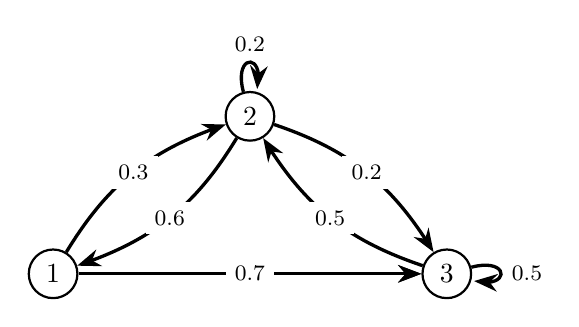
\begin{tikzpicture}
\begin{scope}[every node/.style={circle,thick,draw}]
    \node (A) at (0,0) {1};
    \node (B) at (2.5,2) {2};
    \node (C) at (5,0) {3};

    \end{scope}

\begin{scope}[>={Stealth[black]},
              every node/.style={fill=white,rectangle},
              every edge/.style={draw=black,very thick}]
    \path [->] (A) edge [bend left=20] node[pos=0.5] {\footnotesize{0.3}} (B);
    \path [->] (B) edge [bend left=20] node[pos=0.5] {\footnotesize{0.6}} (A);
    \path [->] (B) edge [bend left=20] node[pos=0.5] {\footnotesize{0.2}} (C);
    \path [->] (C) edge [bend left=20] node[pos=0.5] {\footnotesize{0.5}} (B);
    \path [->] (A) edge (C);
    \path [->] (A) edge node[pos=0.5] {\footnotesize{0.7}} (C);
    \path[<->] (C) edge [loop right] node {\footnotesize{0.5}} ();
    \path[<->] (B) edge [loop above] node {\footnotesize{0.2}} ();
    
    \end{scope}

\end{tikzpicture}
\end{center}


% \begin{equation} \label{eq8}
% \begin{split}
% N_{open1}^{i+1} &=  e^{-\Delta t / \tau_{open}}N_{open1}^{i} + \pr{1 - e^{-\Delta t P_{total}}}N_{closed}^{i} \\ 
% N_{open2}^{i+1} &= \pr{1 - e^{-\Delta t P_{total}}}N_{open2}^{i} + P_{P}\pr{1-e^{-\Delta t / \tau_{open}}}N_{open1}^{i} \\ 
% N_{inactive}^{i+1} &= e^{-\Delta t / \tau_{inact}}N_{inactive}^{i} + \pr{1-P_{P}}\pr{1-e^{-\Delta t / \tau_{open}}}N_{open1}^{i} + e^{-\Delta t P_{P}}N_{open2}^{i}\\
% N_{closed}^{i+1} &= e^{-\Delta t P_{total}}N_{closed}^{i} + \pr{1-e^{\Delta t / \tau_{inact}}}N_{inactive}^{i} \\
% \end{split}
% \end{equation}


Transition matrix: 
\begin{align}
\mathrm{A} =
\begin{bmatrix} %%%%%%%%%%%%%%
0           &  0.3          & 0.7 \\ 
0.6         &  0.2          & 0.2     \\
0           &   0.5         & 0.5    \\ 
\end{bmatrix}
\end{align}


\section{Diffusion}

 Note that in the coming sections, $[f]$ is used to describe the concentration of some molecule $f$. But, this principal can be applied to anything, including the spreading of voltage across some surface. 

\subsection{Forward Euler's} Diffusion is accomplished using some diffusion coefficient ($D_c$) multiplied by some measure of the proportion in one compartment verses another (often $\partial^2 [f]/\partial x^2)$. $D_c$ can be tuned however desired. The important bit is the second derivative of $[f]$ with respect to space. This can be done using the general form of a second derivative, as written below: 

\begin{equation} \label{diff1}
\begin{split}
f'' = \frac{f_{x + 1} - 2f_x + f_{x - 1}}{x^2}
\end{split}
\end{equation}

\bigskip

One may wonder how one would solve for an edge case, as the general form of a second derivative requires three data points. There are some nuances, but in general the solution is simply the first derivative of the non-edge side. That is, since the second derivative is the difference in derivatives, that leaves simply the derivative of one side minus zero. This is like applying a closed end to your surface. You can ponder how to solve for an open end, if that ever arises.\newline

This method has some slight issues in which the $[f]$ can occasionally go negative. The way in which this occurs is stated below (note that now $[f]$ is used instead of $f$ to signify concentration at a value $x$ and time $t$). We can first describe a simplified version of the problem:

\begin{equation} \label{eq8}
\begin{split}
[f]_i & = f_0\exp(-mt) \\
\frac{d[f]}{dt} & = \frac{[f]_{i+1} - [f]_{i}}{\Delta t} = -m[f]_i \\
[f]_{i+1} & = (1-m\Delta t)[f]_i = [f]_i - m\Delta t [f]_i \\
[f]_{i} & = (1-m\Delta t)[f]_{i-1} = (1-m\Delta t)^2[f]_{i-2} \\
[f]_{i} & = (1-m\Delta t)^i[f]_{0} \\
\end{split}
\end{equation}

You can see easily, from this, that if $\Delta t$ is too big, you will abandon the characteristic decay you'd expect from $f_0\exp(-mt)$, and instead get some diverging oscillatory function. How this applies to our interest in diffusion is described below: 

\begin{equation} \label{eq8}
\begin{split}
\frac{[f]^{t+1}_{x} - [f]^{t}_{x}}{\Delta t} &= \frac{[f]^{t}_{x+1} - 2[f]^{t}_x + [f]^{t}_{x - 1}}{x^2}\\
[f]^{t+1}_{x} - [f]^{t}_{x} &= \frac{\Delta t}{x^2} \pr{[f]^{t}_{x+1} - 2[f]^{t}_x + [f]^{t}_{x - 1}} \\
[f]^{t+1}_{x} &= \frac{\Delta t}{x^2} [f]^{t}_{x+1} + \pr{1 - 2\frac{\Delta t}{x^2}}[f]^{t}_x + \frac{\Delta t}{x^2}[f]^{t}_{x - 1} \\
\end{split}
\end{equation}

Therefore, if we want to ensure that the concentration is always positive, we are constrained by: 

\begin{equation} \label{eq8}
\begin{split}
1 - 2\frac{\Delta t}{x^2} & = 0\\
\Delta t & < \frac{x^2}{2}\\
\end{split}
\end{equation}

The relevance of this being that if one were interested in modeling on a very small $\Delta x$, then one would have to use a $\Delta t$ that is not physiological, and thus waste a great deal of computing power in doing so. This can be avoided explicitly using some other methods, discussed next. 

\subsection{Backward Euler's} This form serves to solve the time-scale dilemma by swapping $[f]_{x+1}$, and can be used with any $\Delta t$. Let us consider the same example from above: 

\begin{equation} \label{eq8}
\begin{split}
[f]_i & = f_0\exp(-mt) \\
\frac{d[f]}{dt} & = \frac{[f]_{i+1} - [f]_{i}}{\Delta t} = -m[f]_{i+1} \\
[f]_{i+1} - [f]_{i} & = -m\Delta t[f]_{i+1} \\
[f]_{i+1} & = \frac{1}{1+m\Delta t}[f]_{i} \\
\end{split}
\end{equation}

Naturally, there is no longer a concern of the size of $\Delta t$. Though, one immediate concern is the difficulty of solving your equation for $[f]_{i+1}$. Getting back to the diffusion interest, we now have:

\begin{equation} \label{eq8}
\begin{split}
\frac{[f]^{t+1}_{x} - [f]^{t}_{x}}{\Delta t} &= \frac{[f]^{t+1}_{x+1} - 2[f]^{t+1}_x + [f]^{t+1}_{x - 1}}{x^2}\\
[f]^{t+1}_{x} - [f]^{t}_{x} &= \frac{\Delta t}{x^2} \pr{[f]^{t+1}_{x+1} - 2[f]^{t}_x + [f]^{t-1}_{x - 1}} \\
\end{split}
\end{equation}


Which simply replaces the previous $[f]^{t}_{x}$ with $[f]^{t+1}_{x}$. This leaves us with three unknowns (those being $[f]^{t+1}$ at $x-1,x,x+1$). We must use linear algebra to solve by first rewriting the left and right side as vectors and a matrix in the following way: 

\begin{align}
\vec{[f]}^{t+1} &= \begin{bmatrix}
        [f]^{t+1}_{0} \\
        [f]^{t+1}_{1} \\
        \vdots \\
        [f]^{t+1}_{x}
\end{bmatrix}
; \vec{[f]}^{t} = \begin{bmatrix}
        [f]^{t}_{0} \\
        [f]^{t}_{1} \\
        \vdots \\
        [f]^{t}_{x}
\end{bmatrix}
\end{align}

and 
\begin{align}
\mathrm{A} = \frac{\Delta t}{x^2}
\begin{bmatrix} %%%%%%%%%%%%%%
\dots       &   \dots       & \dots     &   \dots    &   \dots   \\
1           &   -2          & 1         &            &   \vdots    \\
\vdots      &   1           & -2        &   1        &   \vdots   \\   
\vdots      &               & 1         &   -2       &   1    \\
\dots       &   \dots       & \dots     &   \dots    &   \dots    \\
\end{bmatrix}
\end{align}

The corners $1,1$ and $x,x$ were intentionally omitted, as what one desires to do with this is dependent on how they would prefer to treat their edges. As described before in the \textit{Forward Euler's} method, one can use instead of the $(1,-2,1)$ pattern, simply $(\varnothing,-1,1)$ pattern, which signifies a closed edge. Therefore, together now we get: 

\begin{equation} \label{eq8}
\begin{split}
\vec{[f]}^{t+1} - \vec{[f]}^{t} & = \mathrm{A} \vec{[f]}^{t+1} \\
\mathrm{I}\vec{[f]}^{t+1} - \mathrm{A}\vec{[f]}^{t+1} & = \vec{[f]}^{t} \\
\vec{[f]}^{t+1} & = (\mathrm{I} - \mathrm{A})^{-1}\vec{[f]}^{t}
\end{split}
\end{equation}

Where I is the identity matrix. 

\subsubsection{Remarks.} 
Foward Euler's is explicit, and will be preferred whenever the differential equations are non-stiff\footnote{On approximately the same time scale.}. It is the more accurate of the two methods, and can be less computationally intensive if your decay rates are all slow. Backward Euler's is implicit, and can not be used to solve everything, but is doable in most cases. The extra computation required to solve the system of equations more than makes up for potential limitations in your $\Delta t$. 


\part[Physiology]{Physiology
            \vspace{0.2in}
            \begin{center}
            \begin{minipage}[l]{10cm}\small
                Preoccupied with a single leaf, you won't see the tree. Preoccupied with a single tree, you'll miss the entire forest.  \newline
                -- Vagabond by Takehiko Inoue
            \end{minipage}
            \end{center}}

\section{Overview}

It is very important to avoid taking a quantized approach to studying physiology. You'll notice neuroscience majors may know some superb nuances regarding the role of HCN channels in overexcitable neural disorders, like epilepsy. However, they may be totally unaware of their canonical role as pacemakers in the heart. So too may they be unaware of the rich history of modeling $I_h$ currents by computational biologists, preferring to look only at a channel as it functions in neurons. Hence, one must not become preoccupied with a single leaf. 


\chapter{Muscles}

\section{Skeletal Muscle}
\subsection{A Cellular Level}
\subsubsection{Structure.}
Skeletal muscles are composed of muscle fibers, which are composed of myofibrils. Muscles use a silly nomenclature, in which ``sarco" is added to words. For example, the whole structure sits within the sarcoplasm (cytoplasm), fibers are intertwined with the the sarcoplasmic reticulum (equivalent to endoplasmic reticulum) and surrounded by the sarcolemma (equivalent to the cell membrane). An individual myofibril is made up of overlapping actin and myosin segments, held together, to some degree, by titin. The myosin heads are the canonical structure you imagine, which bud off of the end of a chain like leaves on a branch and bind to actin. Undeniably, the most uninteresting part of muscle physiology is as follows: The ``centerline" of the myosin networks is called the M line, while the ``centerline" of the actin network is called a Z disk. Titin branches off from the Z disks to bind to the ends of myosin chains, providing both some elasticity and support for myosin. Actin chains are centered around a line of nebulin, which too provides structural support and organization. The I band is considered to be the unbound part of the actin structure, centered around the Z disks. The H zone is the unbound part of the myosin structure, centered around the M line. The A band is the entire length of the myosin fibers, thereby encapsulating both the bound part of the actin-myosin complex and the H zone, meaning it too is centered around the M line. Therefore, when contraction occurs, the size of the H zone and I band decreases, while the size of the A band stays the same.

\subsubsection{Contraction-relaxation.}
Myosin heads desire to bind to actin, but are blocked by tropomyosin. Ca$^{2+}$ can bind to troponin, bound to tropomyosin, to cause conformational changes resulting in the exposure of the actin to the myosin heads. In doing so, binding can occur, followed by myosin's power stroke. The energy for the stroke comes from hydrolyzing ATP, which had already occured by the time myosin attached to the actin. The powerstroke allows the release of the ADP and P$_i$. ATP then can bind to the empty active site of myosin, which causes the release of the head and prepares it for another cycle. Notably, when ATP does not bind to myosin, the muscle will be stuck in the rigor state.\newline

In skeletal muscles, the source of Ca$^{2+}$ is a combination of the extracellular Ca$^{2+}$ flowing inward, and further release from the sarcoplasmic reticulum. The story goes as follows: a motor neuron releases acetylcholine onto the motor end plate (an area which a high density of sodium channels). This causes a depolarization, which propagates down the muscle fiber. Structures called T-tubulues sink lower into the tissue, allowing for more direct access to the inner processes (visually, these look similar to gyri in the brain or the crypts of the intestinal wall). The T-tubules are lined with dihyropyridine (DHP) channels, an L-type VGCC (specifically Ca$_v$1.1). DHP and ryanodine receptors (RyR) can be mechanically coupled, which influx of Ca$^{2+}$ in through DHP mechanically opens RyR channels of the sarcoplasmic reticulum (a large store of Ca$^{2+}$). The free calcium is lowered through things like active pumping out of the sarcoplasm.\newline

A steady supply of ATP is needed to maintain pumping, and it is said that at any given time, there is 8 or so twitches worth of ATP within the muscle fiber. Therefore, frequent production and alternate stores are required for continuous movement. One such storage is phosphocreatine, whose phosphate group can be quickly transferred to ADP through creatine kinase. Muscles therefore contain high levels of this enzyme, and \textbf{testing for it in the bloodstream can be a good proxy for muscle damage}.\newline

Notably, it is very difficult to fully deplete a muscle of its ATP. Other forms of fatigue begin before this can possibly occur, which include CNS or PNS feedback. An example of this may be that acetylcholine is not synthesized fast enough to continually stimulate muscle fibers. Continual simulation of muscle fibers, beyond what is allowable under normal conditions, \textbf{will fully deplete ATP levels and therefore cause damage to muscles}. Another consideration is the continuous use of ATP may result in P$_i$ buildup in the sarcoplasm, making release of ADP $+$ P$_i$ from myosin less likely to occur. Too, this opens the possibility of calcium phosphate forming, which can be quite damaging if it crystallizes further. There are also ion concentration changes to consider, and continued stimulation can result it tetanus.

\subsection{Nervous system control}

% COMMENTING OUT BECAUSE I AM UNSURE WHAT SECTION TO PUT THIS IN.
% \subsection{Disorders}
% There are many ways one can lose control of their muscles. Nerve damage, for example, will halt the release of acetylcholine onto the motor plate. In a similar manner, botulism is a result of the botulinum toxin blocking release of acetylcholine, resembling the effect of nerve damage. In muscular dystrophy, the protein dystrophin is absent, which would normally attach actin to the cell membrane. Evidently, this can result in membrane permeability, calcium influx, and thus activation of digestive enzymes that breakdown muscle fibers. In McArdle's disease, muscles simply cannot convert glycogen to glucose-6-phosphase, causing the energy supply to be limited. 


\section{Smooth Muscle}

Smooth muscle is much more variable than skeletal, differing by location, contraction pattern, required inputs, and structure. 


\subsection{A Cellular Level}
\subsubsection{Structure.}
Smooth muscle is not considered to have sarcomeres, despite it having the same basic structural components of skeletal muscles. Smooth muscle contains much more aactin than does skeletal muscle, and notably does not contain troponin like skeletal muscle does. Smooth muscle networks are connected through intermediate filaments, which usually attach to dense bodies within the cytoplasm. Actin also attaches to dense bodies, maintaining the actin-myosin network within the cell as well. Smooth muscles do not have T-tubules like skeletal muscles. A comparable structure may be calveolae, which do indent into the membrane and seem spatially associated with the sarcoplasmic reticulum. The autonomic nervous system stimulates fibers through neurotransmitter release from varicosities, or bulbous stores of the chemical. The neurons may innervate the muscle fibers, allowing multiple muscle cells to be stimulated at once, or they may be release to a few fibers, which are connected through gap junctions and stimulate the nearby ones, causing a propagating wave to stimulate others. The first case describes a multi-subunit muscle, and the second a single subunit. 

\subsubsection{Contraction-Relaxation.} 
Initiation of contraction begins the same as skeletal muscle, in that calcium enters and the concentration is further driven up by sarcoplasmic calcium release. Though, in this case Ca$^{2+}$ may enter either through gap junctions or membrane ion channels. As such, there are many more modes of entry than in skeletal muscle. For example, voltage-gated Ca$^{2+}$ channels may open, but there are also ligand gated channels or stretch-activated channels, adding extra layers of possible regulation. Intracellular differences arise beginning from release from the SR. Firstly, is is no longer a mechanically gated RyR channel which allows its release. The release mechanism is now Ca$^{2+}$ activated RyR release (commonly called Ca$^{2+}$-induced-Ca$^{2+}$-release (CICR)), and the IP$_3$ path. GPCRs activate phospholipase C, driving IP$_3$ production which binds to SR channels and causes them to open. The IP$_3$ path is usually considered the greatest way to drive up intracellular Ca$^{2+}$ (or at least, that is what computational biologists seem to think). When Ca$^{2+}$ is available, it binds to calmodulin (CaM), which then binds to the myosin light chain kinase (MLCK). MLCK phosphorylates myosin to increase myosin ATPase activity. Importantly, once contraction occurs, it stays stiff until released by a different mechanism. Because after contraction, no work is being done in the stiff state, smooth muscle is able to stay contracted for long periods. This explains why sphincters in the body are able to stay closed all the time, while one's bicep fatigues after carrying groceries for just a little while. Relaxation begins when Ca$^{2+}$ is either pumped out of the cell through a Ca$^{2+}$ATPase pump, or sodium transporter. This causes CaM to unbind, myosin light chain phosphatase (MLCP) to dephosphorylate myosin, and the myosin heads to release from actin. Interestingly, diacylglycerol (DAG), another product of the IP$_3$ path, inhibits MLCP and thereby enhances muscle contraction.\newline

The calcium stored in the SR is maintained in a number of ways. One example being the protein STIM1 responding to lower Ca$^{2+}$ levels within it, moving toward the cell membrane, and activating store operated Ca$^{2+}$ channels, such as Orai1. 

\subsection{Nervous system control}

\section{Cardiac Muscle}
\subsection{A Cellular Level}
\subsubsection{Structure.}
\subsubsection{Contraction-Relaxation.} 
\subsection{Nervous system control}
\subsection{Pacemakers}





\chapter{The Spinal Cord}

\section{Central Pattern Generation}

Defining the central pattern generator is still somewhat contested. Computational models have been used to explore its existence\footnote{\url{https://www.nature.com/articles/s41598-021-91714-1}}, and for now we should take a few unifying assumptions: \textbf{(1)} the central pattern generator exists and is used to generate rhythmic moving, such as walking, \textbf{(2)} in many cases it is initiated by the CNS, but aside from that is largely devoid from CNS input, and \textbf{(3)} the CNS can work in tandem to compute integrated moving that requires coordination and balance. 

\part[Spinal Cord Injury]{Spinal Cord Injury
            \vspace{0.2in}
            \begin{center}
            \begin{minipage}[l]{10cm}\small
                ?? \\
                -- ??
            \end{minipage}
            \end{center}}

\chapter{The Injury Itself}

Spinal cord injury is composed of the primary injury, prototypically, but not restrictively, due to some kind of high impact action. This is usually unpredictable and highly variable. Secondary injury, resulting from inflammation, oxidative stress, and other biological responses is much more predictable and potentially lends itself better to therapeutic intervention.\newline

The lesion's composition is categorized in three ways: \textbf{(1)} the non-neural core, \textbf{(2)} the astrocytic scar around the core, and \textbf{(3)} the spare reactive neural tissue. In the mix of immune cell influx and scar formation, no neural cells can survive at the center of the lesion. On a neuronal level, the rostral end retracts in a process of Wallerian degeneration. The caudal end dies away. Growth from the cell body is limited both by the damaged cell's biochemistry and by the physical barriers which now present themselves in front of the axons. The physical barriers that immediately succeed injury are often called damaged axon-glia complexes (AGCs). Discussed further later, immune cell influx causes astrocytes to form a scar, meant to save the spare surrounding neural tissue, which is composed of both glia and neurons.\newline

The traditional aim of treatment is to bridge the corticospinal tract with distant neurons through a therapeutic combination of inhibiting anti-regenerative and promoting regenerative factors. As I have commented many times, getting neurons to regenerate alone is insufficient in many cases, as reformation of the correct synapses will not necessarily follow. Forcing axon regeneration alone is, incidentally, not too hard---one can pump neurons full of metabolites or simply implant stem cells. The issue being that they do not know where to grow to. One possible route to solving this is remodeling neural circuits using interneurons to bridge these connections. There are also attempts to use biomaterials to simulate a pro-regenerative environment, hopefully enhancing plasticity of the circuits.\newline


\section{Cell Specific Responses}
The discussion, for the moment, will mostly use information gathered from Hu \textit{et al.} 2023.


\subsection{Immune Response}
As SCI breaks the spine-blood barrier, influx of immune cells can cause further damage. Evidently, the nature of the immune response being helpful or harmful is still largely contested.

\subsubsection{Neutrophils.}
Neutrophils compose part of the immediate response to injury, which are recruited by cytokines and chemokines secreted by cells damaged in the primary injury. They essentially initiate the secondary injury, and reach their peak around 1 DPI. Like most cells, the role of neutrophils cannot be characterize as solely pro- or anti-regenerative. While a high influx of neutrophils is associated with poor patient outcomes, so too are neutrophils associated with guiding macrophages to damaged tissue, suggestive of better recovery. 

\subsubsection{Microglia.}
In mouse SCI models, it seems that there are two peaks of microglial activity. The time course is remarkably long and disparate, reported 7 DPI and 60 DPI. Microglia can either promote inflammation, thereby worsening the secondary injury (called the M1 phenotype) or decrease inflammation, and promote repair (called M2). It is likely that this response depends on the subtype of microglia, which varies depending on the environment. Regardless, it is true that the earlier one treats SCI, the more likely one is to avoid negative microgial effects. Fascinatingly, in a neonatal setting microglia are able to heal SCI almost entirely through their role secreting fibrinogen, which is able to connect damaged axons back together. 

\subsubsection{Macrophages.}
Macrophages are considered to be the dominant immune cell located around the injury site. Microglia, conversely, are scattered around the borders of the injury. Depending on the type of glial scar that is formed, different types of macrophages have been found. Macrophages mediate the corralling\footnote{Corralling is a term used to describe the formation of a barrier around the injury, preventing further injury. It is composed astrocytes, and other cells, and is important in repair.} of cells around the injury site. The phagocyotitic abilities of macrophages are of key importance, as loose fragments of cells must be removed, and microglia are incapable of keeping up such a high demand for removal. As a large part of this includes the destroyed mylein of oligodendrocytes, macrophages uptake great amounts of lipids. This can result in the formation of lipid droplets, which causes macrophages to become ``foamy." This foamy phenotype impairs further repair. 

\subsubsection{Lymphocytes.} 
The adaptive immunity is fairly universally regarded as harmful to regeneration (with some exceptions, of course). T cells further break down the spine-blood barrier and increase immune cell invasion. Evidently, T cell entry is also a major sourse of neuropathic pain in SCI patients. In general, it seems established that the overall immune response after injury impairs further regeneration, and a good example of this can be found here\footnote{\url{https://www.science.org/doi/full/10.1126/science.abd5926}}. 

\subsection{Neural Response}

Apoptosis of neurons initiates at around 4 HAI, but peaks at only 8 HAI\footnote{It is worth noting that these times are likely quite inaccurate, or very injury-type specific. But, they do give a good indication of the approximate timeframe---such as that the majority of this apoptosis occurs within the first day or so after injury.}. 

\subsubsection{Interneurons.}
Fascinatingly, it was shown that the ability of neonatal mice to fully recover from SCI was due, in part, to interneurons maintaining excitatory conditions. In adult mice, these interneurons switch to inhibitory after SCI, which dampens signals to motor neurons. A paper investigating this can be found here\footnote{\url{https://www.nature.com/articles/s41593-022-01067-9}}. One must wonder, can you electronically mimic the excitatory interneurons in fully grown mice? Similar approaches have been done therapeutically, such as with potassium-chloride cotransporter-2 (KCC2) agonist CLP290\footnote{\url{https://www.sciencedirect.com/science/article/pii/S009286741830730X}} which seems to dampen the overexcited, inhibitory interneurons. Perhaps one could simply use something like DBS (or in this case, DSS?) on these interneurons.  

\subsubsection{Astrocytes.}
Astrocytes, being the dominant supportive cell, plays an essential role in SCI. After injury, astrocytes form a physical barrier that is supposedly intended to limit the secondary injury. This occurs after astrocytes become activated, and are helpful in the initial stages but later form a glial scar, impairing regeneration. Astrocytes may either be activated by inflammation, causing them to be neurotoxic (called A1 cells) or by ischemia, causing them to be neuroprotective (A2 cells). The first transformation occuring through the NF-$\kappa$B path, and the second through STAT3. Microglia are said to be the greatest contributor to activating astrocytes through release of signaling molecules. Another important factor is type 1 collagen upregulation, which results in astrocytic adhesion through cadherin, causing activation and eventual scar formation.\newline

The astrocyte scar is surprisingly thin, only a few layers of cells. Though, its importance is not to be underestimated. When ablated, mice with SCI were worse off by almost every metric. A cornerstone paper on the topic seems to be here\footnote{\url{https://www.nature.com/articles/nature17623}}. While scar tissue is primarily astrocytic in origin, it is worth mentioning that pericyte derived scar tissue (sometimes called the fibrotic scar) too play a role. Their positive roles include boosting tissue integrity, but so too do they seem to block axon regeneration as a physical barrier. 

\subsubsection{Oligodendrocytes.}
Oligodendrocytes reportedly begin apoptosis around 1 DPI and it peaks around 8 DPI. Oligodendrocyte precursor cells (OPCs) are may differentiate into oligodendrocytes or Schwann cells after SCI. OPCs have been show to remyelinate neurons after SCI, but fascinatingly, it has been shown that locomotor recovery after SCI does not necessarily require remyelination by oligodendrocytes\footnote{\url{https://www.nature.com/articles/s41467-018-05473-1}}. Though, plenty of other research suggests it is required---so it is likely context dependent. 

 

\section{Side comments} 
This section serves to allow me to comment random things until I find a place for them later.

\begin{enumerate}
    \item Non-neuronal cells secrete a collagen protein (Cthrc1), which is pro-regenerative and affects the ECM\footnote{\url{https://www.cell.com/developmental-cell/pdf/S1534-5807(20)30984-9.pdf}}. 
    \item The ependyma is a source of stem cells, which contributes to glial scar formation after SCI. Connexin (gap junction) signaling between ependymal cells is supposedly a factor involved in their differentiation. 
\end{enumerate}

\chapter{In The Clinic \& Therapeutic Approaches}
Death rates from SCI are still as high as 20\% in some countries. There is a strong age dependence to this, as the probability of walking again after SCI in those older than 50 is much lower than those under.\newline

For this section, I will largely ignore the uninteresting, obvious approaches to axon/neuron regeneration. This includes the often successful implantation of stem cells and or treatment with various neurotrophic factors. While these represent important measures in the field, they are largely intuitive and still face the broad issue of improper circuit reformation.\newline

\subsubsection{Classifying Injury}
One main method of classifying injury and tracking progress of patients is called the American Spinal Injury Association (AISA) impairment scale. AISA scores are broken into the following categories: 

\begin{enumerate}
    \item Grade A: Complete impairment, where there is no motor or sensory information being transmitted below the injury site\footnote{It is not clear to me if this is measured by EMG or movement.}
    \item Grade B: Incomplete impairment, where there is no motor information being transmitted, but some sensory information is preserved. 
    \item Grade C: There is some motor activity preserved, but more than half of the key muscles are too weak to move against gravity (Grade 3 muscles). 
    \item Grade D: A fair amount of motor activity is preserved, where at least half of the key muscles are above muscle Grade 3.
    \item Grade E: There is no impairment at all!
\end{enumerate}

\subsection{Electrical Stimulation}
Fascinatingly, electrical stimulation has been used in conjunction with physical therapy in the past with good resuts\footnote{\url{https://www.nejm.org/doi/pdf/10.1056/NEJMoa1803588?articleTools=true}}. The reasons may be that this promotes stem cell differentiation\footnote{\url{https://www.mdpi.com/2073-4409/11/5/846}}, or disrupts inhibitory interneuron signaling. The optimal electrical application for differentiation has been explored extensively\footnote{\url{https://www.frontiersin.org/articles/10.3389/fbioe.2021.591838/full}}. One may wonder if the benefits of BSI are in the interface itself, or simply the stimulation. Combining stem cell implantation and electronics is, likely, the future.\newline

A slightly different rose by the same name is functional electrical stimulation (FES). Many trials have shown improvement in patients treated with either external stimulation or internal stimulation. 

\subsubsection{Light.}
Light stimulation feels like a footnote in the electrical modulation story, to me. Though, if one wanted to control different neurons or enzymes on an alternate time course, optogenetic activation may be an option. The obvious issue being that one does not have genetic access to patients, and therefore would need to design (likely very complicated) targeted therapeutics. 

\subsubsection{Sound.}
Another footnote is ultrasound simulation. In this case, it will be low intensity focused ultrasound. Some approaches have seen altered gene expression, but perhaps a more promising one is modulating mechanosensitive channels as was shown here\footnote{\url{https://www.nature.com/articles/s41467-022-28040-1}}. Notably, this paper found that many mechanically activated channels are affected in ultrasound, including Piezo, and many of the Trp family proteins. 

\subsubsection{Magnetics.}
I would be extremely curious to know if the magnetic field itself has any unique properties beyond its manipulation of the electric field. Still, too, the story is the same. Some seem to enhance channel activation, while others expression. Interestingly, transcranial magnetic stimulation (TMS) has been used as a treatment with some success. Incomplete spinal cord injury has seen improvements from TMS. 

\subsection{Biomaterials}
The overall goal in the use of biomaterials is to block a worsened immune response, scar formation, and promote neuron activity. Adding promise to stem cell implantation is the use of biomaterials that enhance proper network reformation\footnote{\url{https://pubs.rsc.org/en/content/articlepdf/2022/bm/d1bm01744f}}. Theoretically, a perfect biomaterial could be a substrate preferable for neuron growth, contain molecules that inhibit the immune response, neurotrophic factors that enhance stem cell differentiation and recruitment, and ion channel agonists. Notably, to date there have been no major publications where a ``cocktail" like this has been successful. These sorts of things are usually made from hydrogels, collagens, or select inorganic fibers.\newline

An open question is how one could leverage biomaterials to help clear damaged parts of neurons/cells that would normally be cleared by phagocytosis. Perhaps, one could add materials that are easily oxygenated to dampen the blow of ROS.\newline

To date, implantation of biomaterials have been relatively lackluster in treating patients. While some regeneration scaffolds have proven to improve some neurological function, no patient has regained motor function. 

\subsection{Drug Treatment}
Drug treatment primarily follows the same paths, being reduction of inflammation and neuroprotection. Methylprednisolone (MP) is the only drug approved to treat SCI and works through reducing inflammation. Notably, some side effects have been observed and therefore MP has fallen out of favor for treatment. 

\subsection{Surgery}
I think you'll find that there is a disappointing lack of options---signaling the primitive nature of neurosurgery! Anyway, surgical intervention aims to restabilize the spinal cord as quickly as possible, particularly through decompression. Early surgery seems indicative of shorter ICU stays and better neurological recovery. The first day or so post SCI is the critical time. Interestingly, even after decompression, the pressure within the spine remains high due to fluid build-up within the dura matter. This makes blood reperfusion more difficult, leading to more problems. While durotomy is often a complication of surgery due to progressive CSF leakage after operation, in this case it can be helpful to lessen spinal pressure, which there evidently is a long tradition of\footnote{\url{https://www.sciencedirect.com/science/article/pii/0020138388901325}}. Duroplasty is a more modern and sophisticated alternative, and can allow opening of the dura matter without as much risk\footnote{\url{https://www.liebertpub.com/doi/full/10.1089/neu.2014.3668}}.\newline

Incision directly into the spinal cord itself, myelotomy, has also been done with some success. The belief is that it helps drain some of the harmful dying tissue. There seems to be time dependence in this, where if performed too late after injury it will simply reinvigorate inflammation. 

\subsection{Rehabilitation}
As you would intuit, exercise is the most common technique, as it preserves muscle mass and promotes circuit reorganization. Another rehabilitative technique is pumping in a significant amount of oxygen, as ischemia occurs after injury. BSIs have also become more popular. Fascinatingly, decoding of handwriting has been used to generate text\footnote{\url{https://www.nature.com/articles/s41586-021-03506-2}}. Though, these seem to require deep access to the brain. 

\section{Integrated Approach}
So it seems to me that a good course of treatment would be something like: 

\begin{enumerate}
    \item Immediately after injury, implant a hydrogen with a good restorative milieu, and immunosuppressants.
    \item As microglia peak around a week after injury, a few days later the hydrogel can be removed and stem cell implantation can begin. 
    \item Throughout this time, electrical stimulation can be applied. 
    \item Some time after this, rehabilitation through physical therapy can begin. 
\end{enumerate}


\part[Brain-Spine-Muscle Interfaces]{Brain-Spine Interfaces
            \vspace{0.2in}
            \begin{center}
            \begin{minipage}[l]{10cm}\small
                When we stand at the edge of the ocean, we can not understand its vastness. We know only that it is big. Itt$\overline{\mathrm{o}}$ Ittosai is big. And what about Kojir$\overline{\mathrm{o}}$? \\
                -- Reworded from Vagabond by Takehiko Inoue
            \end{minipage}
            \end{center}}

\chapter{Biochemistry}

While one may find it odd to begin an electronics discussion with a chapter on biochemistry, the fact of the matter is an integrated approach is the only way. As such, to be able to interface with the electrophysiology of neurons, one must fully understand it. 

\section{Ion Channels}



\chapter{The Technology of SCI}

\section{Historical Dealings}

Using electronics to study neural circuits has a long and storied history. One can think of Hodgkin and Huxley, whose ubiquitous nature avoids a need for citation, using an operational amplifier to clamp the voltage of giant squid axons to learn of their properties. In the case of solve spinal cord circuits, so too have electronics long been used\footnote{\url{https://journals.physiology.org/doi/epdf/10.1152/jn.1943.6.2.111}}.\newline

Restoration of the signals which pervade severance in spinal cord injury through therapeutics has been equally explored. For example, drugs such as clonidine, $\alpha_2$ receptor agonist, can promote walking in cats with spinal cord injury\footnote{\url{https://journals.physiology.org/doi/full/10.1152/jn.1998.79.6.2941}}. This effect can be blocked completely by yohimbine, an $\alpha_2$ receptor antagonist\footnote{\url{https://www.ncbi.nlm.nih.gov/pmc/articles/PMC2278596}}.\newline

The ability to generate walking-like movements from electrical stimulation of the lower spine, the T10-L1 region, has been long known\footnote{\url{https://www.sciencedirect.com/science/article/pii/B9780444521378000188}}$^,$\footnote{\url{https://journals.sagepub.com/doi/pdf/10.1177/1073858417699790}}. In these instances, ``tonic" stimulation was able to generate step-like movements. Although the term ``tonic" is dubious because other papers by the same lab identified frequency dependence in their stimulation\footnote{\url{https://link.springer.com/article/10.1007/s00422-004-0511-5}}. While one can generate step-like movements at once frequency, continued extension can be generated with another. 

\section{Reading Thoughts} 

My personal opinion is that the limiting factor in bridging from the stimulation applied by Tator and Minassian is a reliable way to read ones objective through their brain waves. Lorach and the Courtine group solved this using the WIMAGINE system\footnote{\url{https://www.frontiersin.org/articles/10.3389/fnins.2019.00847/full}}. Let's begin by discussing the options. 

\subsection{Different Reading Devices} As you would imagine, there is a tradeoff between the resolution and the damage you will confer upon one's brain. This is described well by Schwartz in 2006, so notably technology may have advanced since then\footnote{\url{https://www.sciencedirect.com/science/article/pii/S0896627306007264}}. The four classes of devices are: 
\begin{enumerate}
    \item Electroencephalography (EEG)
    \item Electrocorticography (ECoG)
    \item Local field potentials (LFPs)
    \item Single Unit AP
\end{enumerate}

EEGs, naturally, are non-invasive and have a reading range on the order of a few centimeters. ECoG is on the tenths of centimeters level, while LPS is millimeters level. Single unit AP is as the name describes, and reads individual action potentials. EEGs sit far above the cortex, outside of the skull, and ECoG come in contact with it. Both LPS and single unit require the electrodes to be buried within the cortex itself, thus causing damage to the brain tissue. Therefore, EEG is typically preferable, as it does not require surgery. It is highlighted by Schwartz that many negatives can occur long term from invasive procedures, such as degeneration, volume displacement, or glial encapsulation. Therefore, it is for this reason that I presume the ability to read ones objective was the limiting factor in progressing the field. \newline

For the moment, I will avoid describing individual technologies between the four groups, as it is likely that the tech progresses greatly each year, and it would be pointless to attempt to describe the reading ranges of any without being totally up-to-date. Instead, we will discuss the WIMAGINE in depth here.

\subsubsection{WIMAGINE ECoG.}
As the name suggests, the device requires the skull to be torn away and must sit directly upon the cortex. It features 64 electrodes, and a human patient would need to have two implanted in order to read both sides of one's motor cortex.\newline

The device was tested longest in sheep, which was a 10 month trial. Surprisingly, at the end of the 10 month trial, through GFAP staining, they still found a great deal of glial migration/build-up around the site. They did not quantify this, but in my personal opinion, this does not bode well for our patient---as they will have to spend a lifetime with the device. Secondly, calcification of the dura matter over the device had begun. This is not inherently surprising, and perhaps is a good sign that the bone was not irreversibly damaged. However, as the device is wirelessly charged, and wirelessly transmits brain information, one must wonder how years of calcium buildup may impact the ability to send or receive information. Too, if the technology needs a dust-up, the surgeons will have to re-destroy these calcified layers. There is quite a lot of fuss made about the fact that the device is wireless, and how it was a decision made to best serve patient comfort. But, in my opinion, it may spell out more long-term harm than good. It is not clear to me yet whether the $8\times 8$ resolution of the electrodes is sufficient to delineate all necessary information. Though, this is the trade-off one must make in choosing between EEG, ECoG, and LPS.\newline

The WIMAGINE system digitizes information with 12 bits of resolution. Data is processed through pwelch spectral analysis. From what I can gather, this is simply another implementation of the FFT. 


\section{Lorach and the Courtine Group} This is the most recent iteration of an ongoing project by the Courtine group. 

\subsection{Overview} The group used surgical implantation into the skull, over the motor cortex, to record patient movements and wirelessly transmit this to the spinal cord. The technology used to capture these electrocorticographic (ECoG) signals is the WIMAGINE. The design features two antennas, and the second of which transmits motor signals that are to be decoded and sent to a pulse generator. The pulse generator is ACTIVA RC, the same that is used in deep brain stimulation (DBS) or pacemakers in the heart. There is no mention of having the patient replace this in future years, but my assumption is that a new battery will require a new surgery in years to come. 


\subsection{Shortcomings} The three shortcomings explicitly mentioned in the \textbf{Introduction} are that \textbf{(1)} one using this BSI must have motion sensors on in order to compensate (a sort of PID controller, perhaps),  \textbf{(2)} that the patient's movement was not perceived as natural, and \textbf{(3)} that there was still considerable hurdles in traversing variable terrain. Many more shortcomings exist than this, and we will go through them below.\newline

\subsubsection{Motion Sensors} I suppose it is obvious why one would use a motion sensor rather than an EMG---as it would be too difficult to discern whether the motion itself, or strength of contraction, is too high using an EMG alone. Still, though, I wonder if this is a feasible alternative. Perhaps one can simply predict motion based on EMG patterns.\newline

The largest drawback, in my opinion, is their desire to make it quickly programmed/calibrated. As with DBS, one would actually prefer longer calibration time. That is, one would be happy to wait a few extra hours or days if it makes their ability to walk improve.\newline

Similarly, they commented that the patient tested was able to walk without the BSI turned on (using crutches) after some time. This signals three things to me, \textbf{(1)} this patient's injury was not, per se, insurmountably severe, \textbf{(2)} the plastic abilities of a damaged spinal cord may be better than we had thought---especially since the patient's injury predated this treatment by 10 years, \textbf{(3)} that there was likely some important tuning being done by the brain-spine endogenous connection (i.e., their BSI was not doing all of the work), and \textbf{(4)} in some cases, no BSI is likely needed at all, and electrical stimulation may be sufficient. This in itself is a quite interesting, alternative patient state. For example, one can imagine a scenario where a patient's brain-spine communication is deeply dampened, but not entirely ceased by damage. Therefore, one would only need amplification of signals as opposed to complete generation of new ones. There may be some of that here. Another comment to make is that their signals are incredibly un-sophisticated, as presented in this paper. That is, they use 16 random electrodes, which do not have connections to synapses themselves. Perhaps this design is to hijack a more reflex-based approach to walking---hence why one can not traverse variable terrain that goes beyond reflexive movement.\newline

A comment regarding the surgery itself: The patient's are having two large, 50mm arrays placed into their skull. Naturally, most would agree to this in order to restore their ability to walk. However, it surprises me that they chose to make the device wireless, given that the surgery is already quite invasive. 

\subsubsection{Seven States} 

Data is processed and used to edit the probability distribution of a Markov chain, which progresses the electrode paddle through seven defined states defined below.

\begin{center}
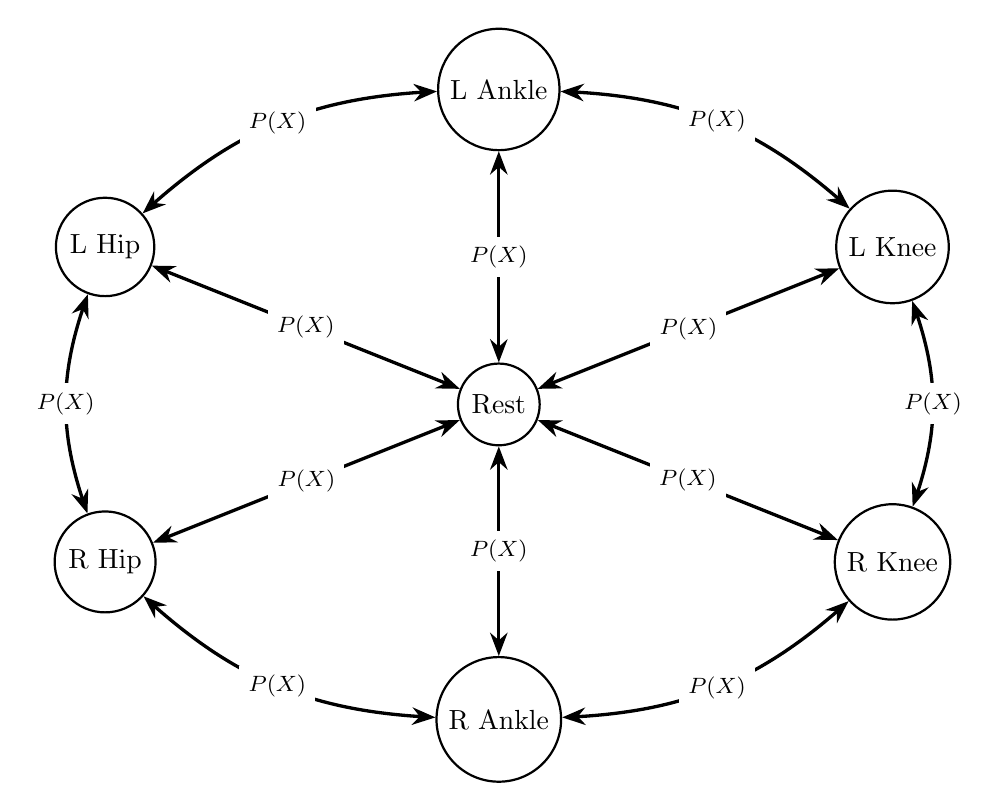
\begin{tikzpicture}
\begin{scope}[every node/.style={circle,thick,draw}]
    \node (Rest) at (0,0) {Rest};
    \node (LeftAnkle) at (0,4) {L Ankle};
    \node (LeftHip) at (-5,2) {L Hip};
    \node (LeftKnee) at (5,2) {L Knee};
    \node (RightAnkle) at (0,-4) {R Ankle};
    \node (RightHip) at (-5,-2) {R Hip};
    \node (RightKnee) at (5,-2) {R Knee};
    \end{scope}

\begin{scope}[>={Stealth[black]},
              every node/.style={fill=white,rectangle},
              every edge/.style={draw=black,very thick}]
    \path [<->] (Rest) edge node[pos=0.5] {\footnotesize{$P(X)$}} (LeftAnkle);
    \path [<->] (Rest) edge node[pos=0.5] {\footnotesize{$P(X)$}} (LeftKnee);
    \path [<->] (Rest) edge node[pos=0.5] {\footnotesize{$P(X)$}} (LeftHip);
    \path [<->] (Rest) edge node[pos=0.5] {\footnotesize{$P(X)$}} (RightHip);
    \path [<->] (Rest) edge node[pos=0.5] {\footnotesize{$P(X)$}} (RightKnee);
    \path [<->] (Rest) edge node[pos=0.5] {\footnotesize{$P(X)$}} (RightAnkle);
    \path [<->] (LeftHip) [bend left=20] edge node[pos=0.5] {\footnotesize{$P(X)$}} (LeftAnkle);
    \path [<->] (LeftHip) [bend right=20] edge node[pos=0.5] {\footnotesize{$P(X)$}} (RightHip);
    \path [<->] (RightHip) [bend right=20] edge node[pos=0.5] {\footnotesize{$P(X)$}} (RightAnkle);
    \path [<->] (RightAnkle) [bend right=20] edge node[pos=0.5] {\footnotesize{$P(X)$}} (RightKnee);
    \path [<->] (RightKnee) [bend right=20] edge node[pos=0.5] {\footnotesize{$P(X)$}} (LeftKnee);
    \path [<->] (LeftKnee) [bend right=20] edge node[pos=0.5] {\footnotesize{$P(X)$}} (LeftAnkle);
    \end{scope}

\end{tikzpicture}
\end{center}

Notably, they did not explicitly mention that one of the progressions could be from state to self state, but one can only assume this is true. So too, only seven states seems to limit the mobility of a patient. 

\end{document}